\begin{figure}[htb]
    \centering
    \begin{subfigure}[t]{0.48\linewidth}{\footnotesize
        \begin{forest}
            for tree={
                circle, draw,
                minimum size=2em
            }
            [16, very thick, label=1
                [11,  label=2
                    [10,  label=4
                        [1, for ancestors={edge=very thick}, edge=very thick,  label=8]
                        [2,  label=9]
                    ]
                    [5,  label=5
                        [4,  label=10]
                        [,color=white, edge=white]
                    ]
                ]
                [9,  label=3
                    [6,  label=6]
                    [8,  label=7]
                ]
            ]
        \end{forest}

        \subcaption{Der Wurzelknoten und die Kanten entlang eines der längsten, einfachen Wege zu einem Blattknoten sind fett gedruckt. Die Anzahl der hervorgehobenen Kanten entspricht der Höhe $h = 3$ des Baums. \label{fig:heap-tree-view}}
    }\end{subfigure}\hfill
    \begin{subfigure}[t]{0.48\linewidth}{\footnotesize
        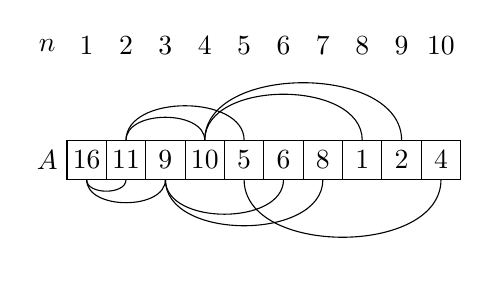
\begin{tikzpicture}
            \path node at (-0.25, 1.25) [] {$A$};
        
            \draw (0.0, 1.0) rectangle (0.5, 1.5) node[midway]{16};
            \draw (0.5, 1.0) rectangle (1.0, 1.5) node[midway]{11};
            \draw (1.0, 1.0) rectangle (1.5, 1.5) node[midway]{9};
            \draw (1.5, 1.0) rectangle (2.0, 1.5) node[midway]{10};
            \draw (2.0, 1.0) rectangle (2.5, 1.5) node[midway]{5};
            \draw (2.5, 1.0) rectangle (3.0, 1.5) node[midway]{6};
            \draw (3.0, 1.0) rectangle (3.5, 1.5) node[midway]{8};
            \draw (3.5, 1.0) rectangle (4.0, 1.5) node[midway]{1};
            \draw (4.0, 1.0) rectangle (4.5, 1.5) node[midway]{2};
            \draw (4.5, 1.0) rectangle (5.0, 1.5) node[midway]{4};

            \draw []   (0.25, 1.0) to[out=-90,in=-90] (0.75, 1.0);
            \draw []   (0.25, 1.0) to[out=-90,in=-90] (1.25, 1.0);
            \draw []   (0.75, 1.5) to[out=90,in=90] (1.75, 1.5);
            \draw []   (0.75, 1.5) to[out=90,in=90] (2.25, 1.5);
            \draw []   (1.25, 1.0) to[out=-90,in=-90] (2.75, 1.0);
            \draw []   (1.25, 1.0) to[out=-90,in=-90] (3.25, 1.0);
            \draw []   (1.75, 1.5) to[out=90,in=90] (3.75, 1.5);
            \draw []   (1.75, 1.5) to[out=90,in=90] (4.25, 1.5);
            \draw []   (2.25, 1.0) to[out=-90,in=-90] (4.75, 1.0);
            
            \path   node at (-0.25, 2.7) [] {$n$}
                    node at (0.25, 2.7) [] {1}
                    node at (0.75, 2.7) [] {2}
                    node at (1.25, 2.7) [] {3}
                    node at (1.75, 2.7) [] {4}
                    node at (2.25, 2.7) [] {5}
                    node at (2.75, 2.7) [] {6}
                    node at (3.25, 2.7) [] {7}
                    node at (3.75, 2.7) [] {8}
                    node at (4.25, 2.7) [] {9}
                    node at (4.75, 2.7) [] {10};
        \end{tikzpicture}
        
        \subcaption{Die Linien über und unter dem Array stellen die Eltern-Kind-Beziehungen zwischen den Knoten dar, Eltern sind immer links von ihren Kindern. \label{fig:heap-array-view}}
    }\end{subfigure}
    \caption{Ein binärer Max-Heap, dargestellt \subref{fig:heap-tree-view} als Binärbaum und \subref{fig:heap-array-view} als Array (wobei $\attrib{A}{heap-size}$ gleich $\attrib{A}{length}$ ist). Die Zahlen in den Kreisen und Rechtecken ist der Wert dieses Knotens beziehungsweise dieses Elements, die Zahlen darüber sind der Index des jeweiligen Knotens/Elements im Array. Angelehnt an \cite[152]{clrs2001} und \cite[88]{ahu1974}.}
    \label{fig:heap-tree-array-view}
\end{figure}